\begin{figure}
\centering
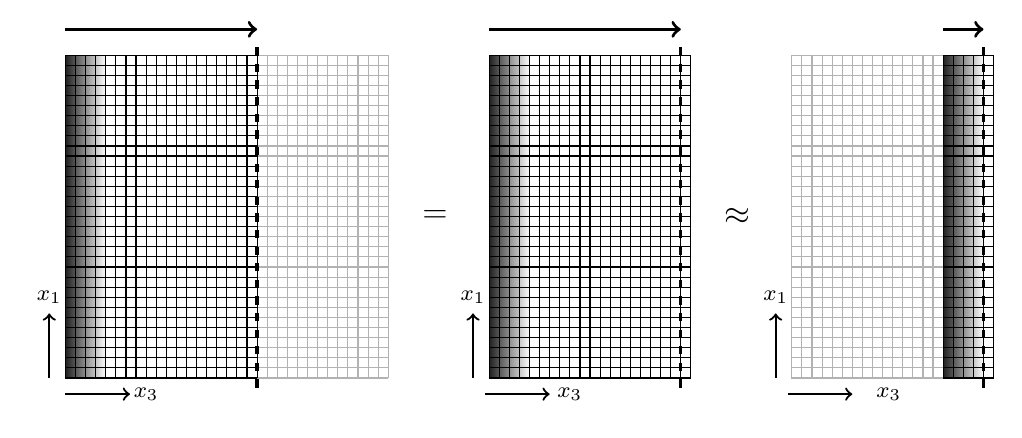
\begin{tikzpicture}[scale=4.1]
\tikzstyle{every node}=[font=\footnotesize]

%
% Draw the left figure
%

% Draw a large arrow showing the direction of the sweep
%\draw[->,very thick] (0.03125,1.08) -- (0.59375,1.08);
\draw[->,very thick] (0,1.08) -- (0.59375,1.08);

% Draw the axes
\draw[->,thick] (-0.05,0) -- (-0.05,0.2);
\draw (-0.05,0.25) node {$x_1$};
\draw[->,thick] (0,-0.05) -- (0.2,-0.05);
\draw (0.25,-0.05) node {$x_3$};

% Fill in the PML regions
\shade[left color=black!87!,inner color=gray,right color=white] 
  (0,0) rectangle (0.125,1);

% Left half of box, (0,0.59375) x (0,1)
\draw[step=0.03125] (0,0) grid (0.59375,1);

% Right half of box, (0.59375,1) x (0,1)
\draw[step=0.03125,opacity=0.3] (0.59375,0) grid (1,1);

% Draw a thick line marking the i'th plane
\draw[very thick,dashed] (0.59375,-0.03) -- (0.59375,1.03);

% Make the PML label
%\draw (0.0625,0.5) node[fill=gray!5!] {PML};

%
% Draw the connection to the middle problem
%

\draw (1.145,0.5) node {\large $=$};

%
% Draw the middle figure (shift right by 1.3125)
%

% Draw a large arrow showing the direction of the sweep
%\draw[->,very thick] (1.34375,1.08) -- (1.90625,1.08);
\draw[->,very thick] (1.3125,1.08) -- (1.90625,1.08);

% Draw the axes
\draw[->,thick] (1.2625,0) -- (1.2625,0.2);
\draw (1.2625,0.25) node {$x_1$};
\draw[->,thick] (1.3,-0.05) -- (1.5,-0.05);
\draw (1.5625,-0.05) node {$x_3$};

% Fill in the PML regions
\shade[left color=black!87!,inner color=gray,right color=white] 
  (1.3125,0) rectangle (1.4375,1);

% Left half of box, (0,0.625) x (0,1)
%\draw[step=0.03125] (1.3125,0) grid (1.9375,1);
\draw[step=0.03125] (1.3120,0) grid (1.9375,1);

% Draw a thick line marking the i'th plane
\draw[very thick,dashed] (1.90625,-0.03) -- (1.90625,1.03);

% Make the PML label
%\draw (1.3625,0.5) node[fill=gray!5!] {PML};

%
% Draw the connection to the right problem
%

\draw (2.0825,0.5) node {\large $\approx$};

%
% Draw the approximate auxiliary problem (shift by 2.25 or 0.938)
%

% Draw a large arrow showing the direction of the sweep
%\draw[->,very thick] (2.7500,1.08) -- (2.84375,1.08);
\draw[->,very thick] (2.71875,1.08) -- (2.84375,1.08);

% Draw the axes
\draw[->,thick] (2.2,0) -- (2.2,0.2);
\draw (2.2,0.25) node {$x_1$};
\draw[->,thick] (2.2375,-0.05) -- (2.4375,-0.05);
\draw (2.55,-0.05) node {$x_3$};

% Fill in the opaque original grid
%\draw[opacity=0.3,step=0.03125] (2.25,0) grid (2.8755,1);
\draw[opacity=0.3,step=0.03125] (2.249,0) grid (2.8755,1);

% Fill in the PML regions
\shade[left color=black!87!,inner color=gray,right color=white] 
  (2.71875,0) rectangle (2.84375,1);

% Left half of box
%\draw[step=0.03125] (2.71875,0) grid (2.875,1);
\draw[step=0.03125] (2.7187,0) grid (2.875,1);

% Draw a thick line marking the i'th plane
\draw[very thick,dashed] (2.84375,-0.03) -- (2.84375,1.03);

% Make the PML label
%\draw (2.78125,0.5) node[fill=gray!5!] {PML};

\end{tikzpicture}
\caption{(Left) A depiction of the portion of the domain involved in the 
computation of the Schur complement of an $x_1 x_2$ plane 
(marked with the dashed line)
with respect to all of the planes to its left during execution of 
Alg.~\ref{alg:naive-fact}. (Middle) An equivalent auxiliary
problem which generates the same Schur complement; the original domain is 
truncated just to the right of the marked plane and a homogeneous Dirichlet 
boundary condition is placed on the cut.
(Right) A local auxiliary problem for generating an approximation to the 
relevant Schur complement; the radiation boundary condition of the exact
auxiliary problem is moved next to the marked plane.}
\label{fig:auxiliary}
\end{figure}
